\documentclass[12pt]{article}
\setlength{\oddsidemargin}{0in}
\setlength{\evensidemargin}{0in}
\setlength{\textwidth}{6.5in}
\setlength{\parindent}{0in}
\setlength{\parskip}{\baselineskip}
\usepackage{amsmath,amsfonts,amssymb}
\usepackage{graphicx}
\usepackage[]{algorithmicx}
\graphicspath{ {./images/} }
\usepackage{fancyhdr}
\pagestyle{fancy}

%\usepackage{hyperref}


\setlength{\headsep}{36pt}

\begin{document}

\lhead{{\bf CSCI 3104, Algorithms \\ Explain-It-Back 5} }
\rhead{Name: \fbox{Keaton Whitehead} \\ ID: \fbox{104668391} \\ {\bf Profs.\ Grochow \& Layer\\ Spring 2019, CU-Boulder}}
\renewcommand{\headrulewidth}{0.5pt}

\phantom{Test}
Your social science colleagues are interested in quantifying the differences in
the news sources of ``distant'' groups. Their data is from a social network and
consists of users and their friends. Part of their research involves
quantifying the ``maximum social distance'' of individuals. To accomplish they
need an algorithm that takes in two users as input and returns the maximum
number of social groups that connects them. They propose using a friend of a
friend (FOAF) approach ({\tt foaf()} below) that starts with one of the input
users, finds their FOAFs, then selects the FOAF who has the largest number of
friends in common. For example, in the figure below the user (grey) has four
friends and four FOAFs. One FOAF (black) has 2 friends in common and that user
is selected.  This process repeated for each FOAF until the second input user
is one of the FOAFs. We can assume that a path between any two users exists.
% ----- FIGURE -----
\begin{figure}[h!]
\begin{center}
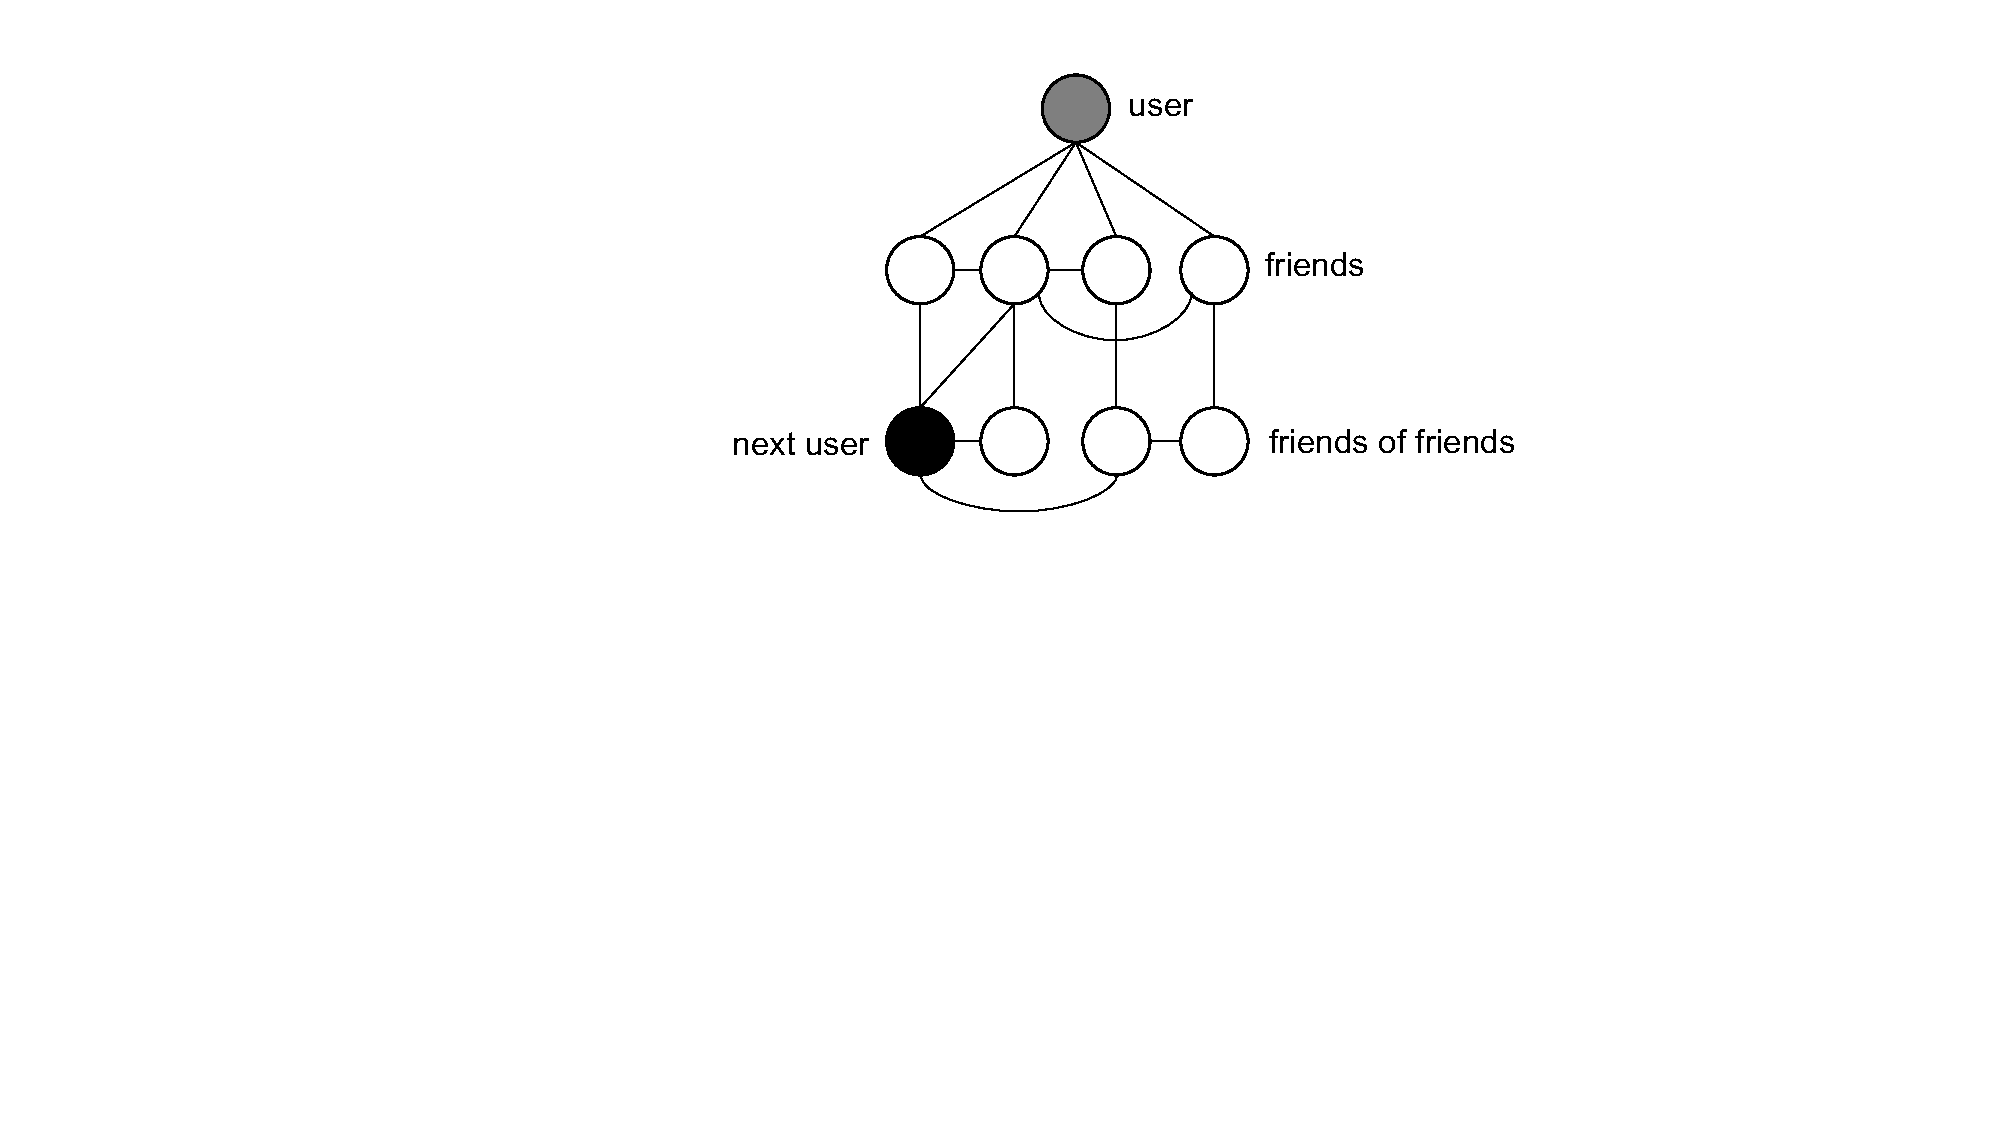
\includegraphics[scale=0.5]{EIB6_graph}
%An undirected graph representing a triangle: $V=\{1,2,3\}$ and $E=\{(1,2),(1,3),(2,3)\}$
\end{center}
\end{figure}
% ----------
\begin{small}
\begin{verbatim}
foaf(user_1, user_2, d):
  F = fiends(user_1) // set user who are friends with user_1
  if user_2 is in F: return d
  FOAF = []
  for f in F:
    FOAF.append(friends(f) - F) // set subtraction
  max_foaf_count = 0
  max_foaf = NULL
  for f in FOAF:
    foaf_count = | intersect(F,fiends(f)) |
    if max_foaf_count < foaf_count:
      max_foaf_count = foaf_count
      max_foaf = f
  foaf(max_foaf, user_2, d+1)
\end{verbatim}
\end{small}
\pagebreak
They seem surprised that, while the algorithm is very fast and give reasonable
results in most cases, every once in a while the algorithm returns a distance
that is different than they expected. Help them understand what assumptions
required for the algorithm they developed and why those are not met here.\\

Hello fellow Social Scientists,\\
\\
I can see why your algorithm seems to work efficiently but results in a few errors. After analyzing your code I noticed a simple problem that you guys have. On the line where you coded: FOAF.append(friends(f)-F) you forgot to incorporate the elimination of the original user from the data set. The problem with this is that you can not be friends with yourself and your code allows this which is why it returns unexpected distances. To help understand this I will give you an example. Let's start with our first individual and we can call him Bob. Bob is in high school and is very popular so he has a lot of friends. He also plays football but his school doesn't offer it so he plays at a different high school. After being on the football team for a while Bob manages to make more friends and this expands his social network. Now, not all of Bob's friends from high school know his football friends to the point that they are considered friends. So if we use your algorithm as it currently stands we will go through all of Bob's friends and find the few that do happen to know each other even though they are in different social networks. Now the problem with your code is because it does not delete Bob, every friend that Bob has is also a friend of Bob, so it is a two-way street. Basically all of Bob's friends have Bob in common which is why they are being counted. If you change this to either eliminate Bob before you compare the friends or make the comparisons only one directional then it should fix this problem. If this is at all confusing or you would like me to elaborate on it more please feel free to message me back. \\
I hope you found this helpful,\\
\\
Keaton Whitehead

\pagebreak

\end{document}
